\documentclass{article}
\usepackage{graphicx} % Required for inserting images
\usepackage[top=0.9in, bottom=1in, left=1.5in, right=1.5in]{geometry}
\usepackage[utf8]{inputenc}
\usepackage[icelandic]{babel}
\usepackage[T1]{fontenc}
\usepackage[sc]{mathpazo}
\usepackage[parfill]{parskip}
\renewcommand{\baselinestretch}{1.2}
\usepackage{booktabs,tabularx}
\usepackage{multirow}
\usepackage{enumerate}
\usepackage{adjustbox}
\usepackage{multicol}
\usepackage{xcolor}
\usepackage{algpseudocode}
\usepackage{tikz}
\usepackage{nicefrac}
\usepackage{changepage}
\usetikzlibrary{arrows, positioning, calc, graphs}
\usepackage{amsmath, amsfonts, amssymb, amsthm}
\usepackage{graphicx}
\usepackage{tikz}
\usepackage{minted}
\usemintedstyle{manni}
\title{Forritunarmál Hópverkefni 10}
\author{Ragnar Björn Ingvarsson, rbi3 \\
		Daníel Snær Halldórsson, dsh11 \\
		Ólafur Sær Sigursteinsson, oss27 \\
	    Elías Ver Bjarnason, evb17 \\
		Helga Björg Helgadóttir, hbh54 \\
	    Eygló Ástþórsdóttir, eya19 \\
	    Kristín Fríða Sigurborgardóttir, kfs14}
\tikzset{->, >=stealth', shorten >=1pt, node distance=2cm,thick, main node/.style={circle,draw,minimum size=3em}}

\begin{document}
\renewcommand\thepage{}

	\maketitle

	\newpage
	\setcounter{page}{1}
	\renewcommand\thepage{\arabic{page}}

	\section{}
	\begin{minted}{haskell}
-- Notkun: hopverk1 x
-- Fyrir:  x er listi [x1,x2,...,xN] af hvaða
--         tagi sem er.
-- Gildi:  Listinn [[xN],...,[x2],[x1]]
hopverk1 x = foldl (\a b -> [b]:a) [] x
    \end{minted}
	\vspace{.5em}
	\begin{center}
		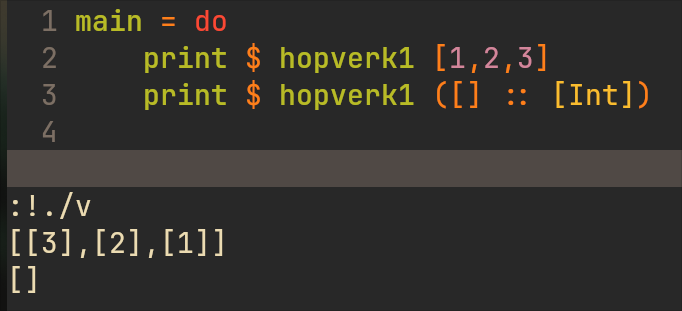
\includegraphics[scale=.35]{h1.png}
	\end{center}
	Ég segi haskell hérna að nota \texttt{[Int]} sem týpu fyrir 
	tóma listann því annars veit það ekki hvernig á að prenta niðurstöðuna.
	
	\section{}
	\begin{minted}{haskell}
-- Notkun: hopverk2 x
-- Fyrir:  x er listi lista af fleytitölum.
-- Gildi:  Margfeldi af summunum af gildum innri lista x.
hopverk2 x = foldl (*) 1.0 (map (foldl (+) 0.0) x)
    \end{minted}
	\vspace{.5em}
	\begin{center}
		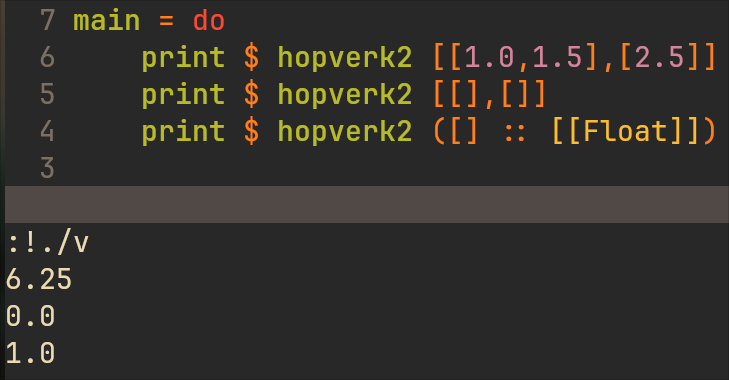
\includegraphics[scale=.35]{h2.png}
	\end{center}

	Ég segi haskell hérna að nota \texttt{[[Float]]} sem týpu fyrir 
	tóma listann því annars veit það ekki hvernig á að prenta niðurstöðuna.
\end{document}
